\begin{frame}[t]{Физиология на невроните}
  Поддържане на различна концентрация на йони в цитозола спрямо околната тъкан.
  \ce{K+} и някои белтъци с общ отрицателен заряд са с по-голяма концентрация в клетката,
  докато \ce{Na+} и \ce{Cl-} извън нея. Това води до създаването на тъй наречения (транс-)мембранен потенциал.
  Клетъчната мембрана се състои основно от липиди, чиято хидрофобна част се държи като диелектрик.
  Липидната част на мембраната всъщност се оказва кондензатор. 
  Предвижването на йони през мембраната става чрез помпи (активно) и канали (пасивно). 
  Основни са тъй наречените натриево-калиевите помпи, това са молекули \ce{Na-K-ATPase}. Те предвижват 3 \ce{Na+} йона навън и 2 \ce{K+} навътре. 
  Други важни помпи са натриево-калциевите, като предвижват 1 \ce{Ca2+} йон навън и 3 \ce{K+} навътре.
\end{frame}

\begin{frame}[t]{Причината за трансмембранния потенциал}
  \begin{figure}[htbp!]
    \centering
    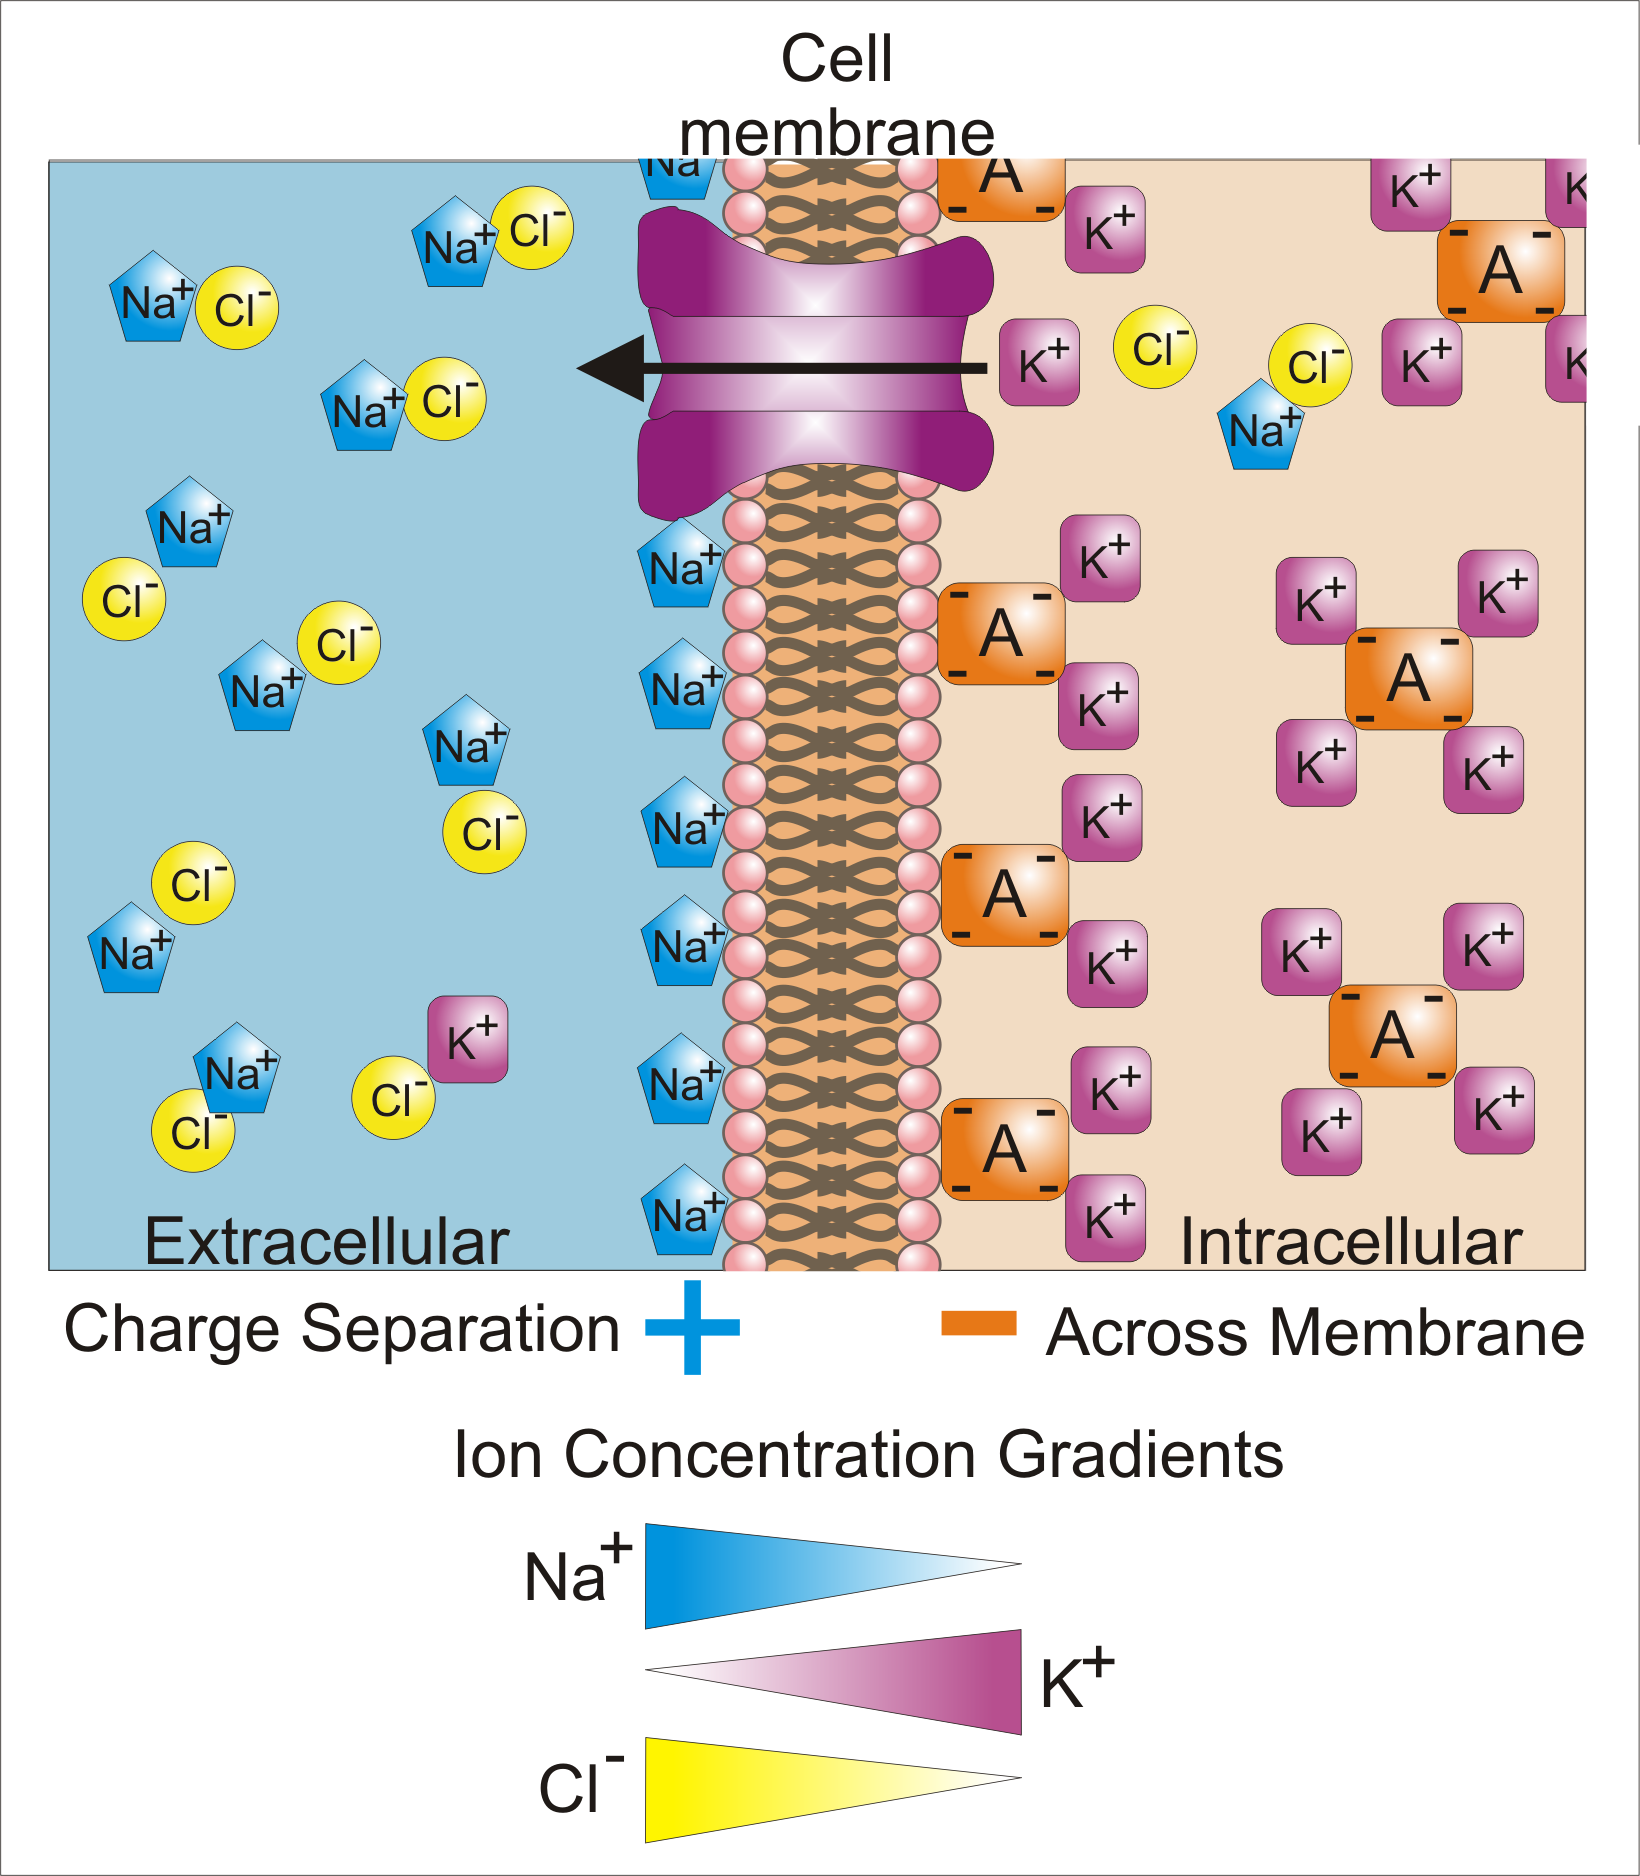
\includegraphics[width=\textwidth,height=0.7\textheight,keepaspectratio]{membrane-potential.png}
    \caption{Йони в цитозола и междуклетъчното пространство от Wikipedia}
  \end{figure}
\end{frame}

\begin{frame}[t]{Физиология на невроните}
  \begin{figure}[htbp!]
    \centering
    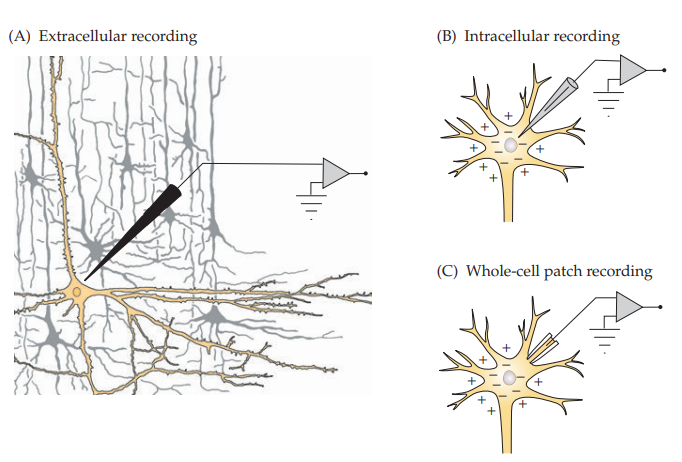
\includegraphics[width=\textwidth,height=0.7\textheight,keepaspectratio]{electrical-recording.PNG}
    \caption{Измерване на потенциала. \cite[Фиг 1.7]{Neuron}}
  \end{figure}
\end{frame}

\begin{frame}[t]{Физиология на невроните}
  \begin{figure}[htbp!]
    \centering
    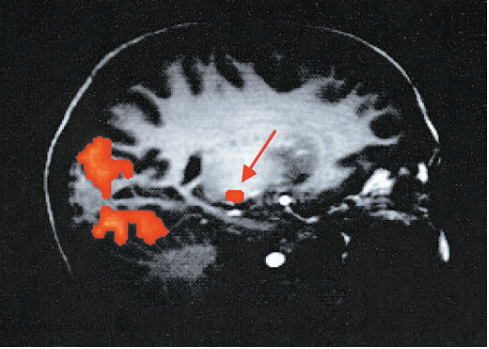
\includegraphics[width=\textwidth,height=0.7\textheight,keepaspectratio]{mri-recording.PNG}
    \caption{Измерване на активността на невроните в главния мозък чрез ЯМР. \cite[Фиг 1.9]{Neuron}}
  \end{figure}
\end{frame}

\begin{frame}[t]{Междуневронна комуникация}
  Предаване на сигнали между неврони става през синапсите. 
  При електричните синапси става директно, едната клетка "продължава" в другата.
  При химическите синапси се образуват везикули (балончета с вещества) в синаптичния цитозол, 
  които се придвижват до мембраната и освобождават вътрешността си в междуклетачното пространство. 
  В резултат следващия неврон може или да бъде възбуден, или инхибиран.
\end{frame}

\begin{frame}[t]{Междуневронна комуникация}
  \begin{figure}[htbp!]
    \centering
    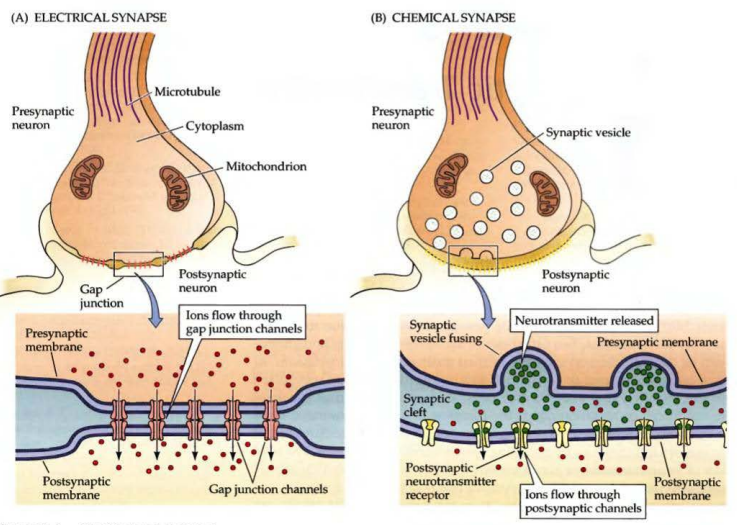
\includegraphics[width=\textwidth,height=0.7\textheight,keepaspectratio]{synapse-types.PNG}
    \caption{Двата вида синапси. \cite[Фиг 5.1]{Neuroscience}}
  \end{figure}
\end{frame}

\begin{frame}[t]{Междуневронна комуникация}
  \begin{figure}[htbp!]
    \centering
    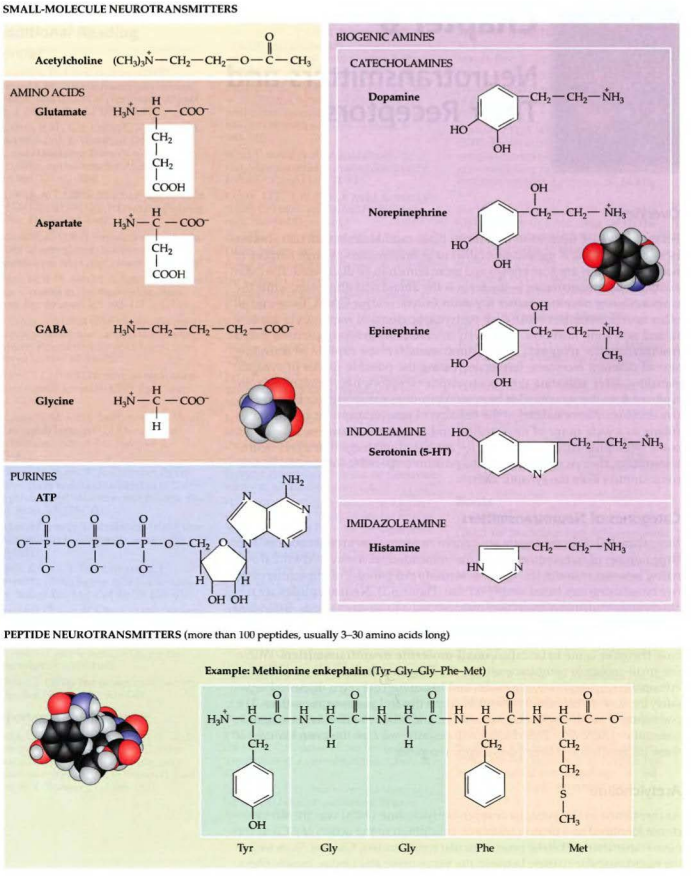
\includegraphics[width=\textwidth,height=0.7\textheight,keepaspectratio]{neurotransmitters.PNG}
    \caption{Молекулите на някои невротрансмитери. \cite[Фиг 6.1]{Neuroscience}}
  \end{figure}
\end{frame}

\begin{frame}[t]{Междуневронна комуникация}
  \begin{figure}[htbp!]
    \centering
    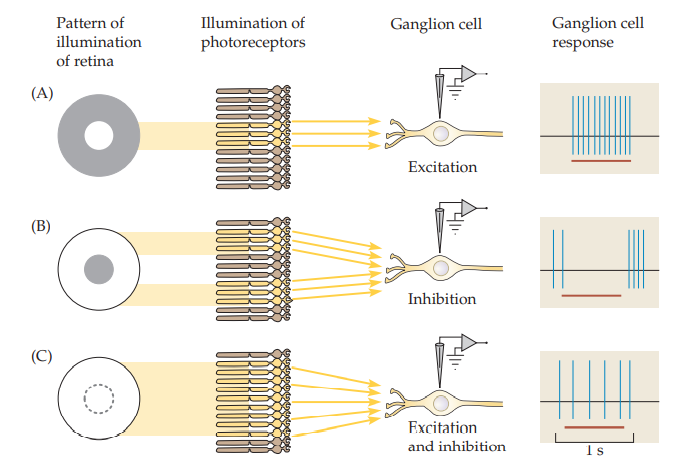
\includegraphics[width=\textwidth,height=0.7\textheight,keepaspectratio]{gangleon-integration.PNG}
    \caption{Интегриране от ганглийна клетка. \cite[Фиг 1.16]{Neuron}}
  \end{figure}
\end{frame}

\begin{frame}[t]{Нервен импулс}
  \begin{figure}[htbp!]
    \centering
    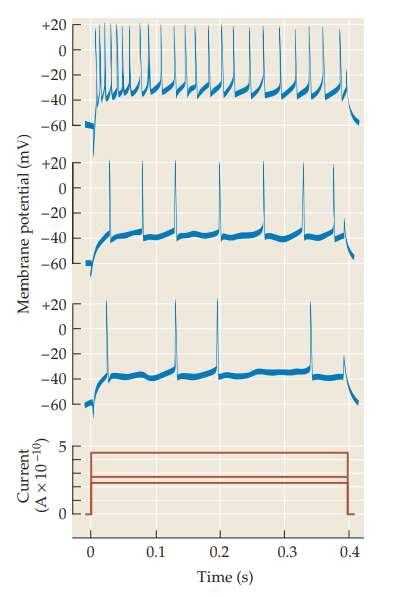
\includegraphics[width=\textwidth,height=0.7\textheight,keepaspectratio]{ac-current.PNG}
    \caption{Резултат от подаване на прав ток чрез електрод в цитозола на ретинална ганглийна клетка. \cite[Фиг 1.12]{Neuron}}
  \end{figure}
\end{frame}

\begin{frame}[t]{Причина за нервния импулс}
  Нервният импулс е резултат от каскадно действие на мембранните канали и помпи.
  Първо клетката се активизира. 
  Ако е рецептор, то тя се възбужда от околната среда.
  В противен случай възбудата става в следствие на получени невротрансмитери от дендритите.  
  След леко повишаване на трансмембранния потенциал се отключват \ce{Na+} канали, чиято ориентация зависи от потенциала (открити благодарение на изследванията на Hodgkin и Huxley).
  %В клетката излизат \ce{Ca2+} и влизат \ce{Na+}, което води до промяна на потенциала и активиране на \ce{Na+} канали, зависими от него.
    %\ce{Na-K-ATPase}.
  %Това води до още промяна на потенциала в околност на натриево-калиевата помпа, което активира други около нея.
\end{frame}

\begin{frame}[t]{Причина за нервния импулс}
  Така потенциала се увеличава още повече и се активизират други канали в околността. 
  Включват се и канали, позволяващи преминаването на \ce{K+} навън.
  След деполяризация каналите се затварят. 
  \ce{Na-K-ATPase} се грижи концентрациите на йоните да се възвърнат първоначалните си стойности. 
  Така потенциала се понижава до достигане (и леко прехвърляне) на стойността му в покой.
  Накрая бавно се достига равновесното състояние.
\end{frame}